% declare our document type
\documentclass[12pt]{extarticle}

%%%%%%%% PACKAGES NEEDED FOR THIS DOCUMENT

% allow us to put pictures in the document
\usepackage{graphicx}
% this line lets us use larger fonts
\usepackage{extsizes}
% this allows us to create ''slides'' in the document
\usepackage[many]{tcolorbox}
% this line lets us caption images inside the ''slides''
% this is neccesary since the slide doesn't allow the use of
% \figure{} inside
\usepackage{caption}
% allows use of courier font
\usepackage{courier}
% make the table of contents links like people are used to
% the hidelinks parts hides link outlines
\usepackage[hidelinks]{hyperref}
% resize the margins
\usepackage[margin=1in]{geometry}
% use utf8 encoding
\usepackage[utf8]{inputenc}
% one of the other packages complained until I put this here
\usepackage[english]{babel}
% allow citations
\usepackage{cite}
% code listings
\usepackage{listings}
% fix single quote in listings
\usepackage{textcomp}

\usepackage{enumerate}

\usepackage[T1]{fontenc}

%%%%%%%%%%% CUSTOM ENVIRONMENT SETUP

% declare a typesetting environment for code/emphasis
\newcommand{\code}[1]{\texttt{\bfseries#1}}
\newenvironment{codeblock}{\bfseries\texttt\bgroup}{\egroup\par}
% better declaration of font environment
%\DeclareTextFontCommand{\codetext}[1]{\code{#1}}
% declare a large font environment for use in the ''slides''
\newcommand{\instruction}[1]{\Large{#1}}
% font environment again
%\DeclareTextFontCommand{\instruction}{\instructionfont}
\newenvironment{instructionblock}{\Large\bgroup}{\egroup}
% declare a ''slide'' text box for use in the document
% the slide is a numbered \section{}
\newtcolorbox[auto counter]{slide}[3][]{%
colback=brown!5!white,colframe=brown!80!gray,height=3.72in,
title={\addcontentsline{toc}{section}{\thetcbcounter ~~ #2}\bf\Large\thetcbcounter ~ #2\hfill #3 \label{slide \thetcbcounter}\setcounter{section}{\thetcbcounter}}}
% declare a ''subslide'' text box for use in the document
% the subslide is a numbered \subsection{}
\newtcolorbox[auto counter,number within=section]{subslide}[3][]{%
colback=brown!5!white,colframe=brown!80!gray,height=3.72in,
title={\addcontentsline{toc}{subsection}{\thetcbcounter ~~ #2}\bf\Large\thetcbcounter ~ #2\hfill #3 \label{slide \thetcbcounter}}}
\renewcommand{\labelitemii}{$\circ$}
\lstset{
	basicstyle=\ttfamily,
	keywordstyle=\bfseries\color{blue!80!black},
	identifierstyle=\bfseries,
	stringstyle=\color{red},
	showstringspaces=false,
	commentstyle=\itshape\color{green!40!black},
	upquote=true
	}

% My Environments (keep these)
\newcommand{\ben}{\begin{enumerate}}
\newcommand{\een}{\end{enumerate}}
\newcommand{\bi}{\begin{itemize}}
\newcommand{\ei}{\end{itemize}}

\newcounter{questionEnumerate}

%%%%%%%%% SET UP OUR TITLE PAGE

\begin{document}
	\title{ Capture -- Filter -- Dissect \\ \large Network Protocol Analysis with Wireshark}
	\author{Created by: Jon Meyer and Jared Zook\\
			Modified by: Ananth Jillepalli, Robert Breckenridge, and Matthew Holman}
	\date{July 1st, 2017 \\ \hyperref[changelog]{Version 3.2}}
	\renewcommand{\abstractname}{Summary}
	\begin{titlepage}
		\maketitle
		\pagenumbering{gobble}
		\begin{center}
			
\includegraphics[scale=.5]{UofI}
			
			\large{CS 439/539: Applied Security Concepts}
			
			\vskip 40pt
		\end{center}
		\begin{abstract}
			Wireshark is a tool for capturing, analyzing and dissecting network traffic. Originally named Ethereal, Wireshark is built upon the \texttt{libpcap} library or equivalent libraries on certain non-Unix based systems. This tutorial provides an overview of Wireshark and an explanation of how it is a powerful tool for network traffic analysis. The process of packet capturing, filtering, and analysis is laid out in a series of demonstrations and walkthroughs. Three challenge questions at the end provide an opportunity to explore Wireshark's functionality on an individual basis.
		\end{abstract}
		\vfill
		\begin{center}
			
\includegraphics[scale=0.5]{cc}
			\vskip 10pt
			This work is licensed under a \href{https://creativecommons.org/licenses/by/4.0/}{Creative Commons Attribution 4.0 International License}.
		\end{center}
	\end{titlepage}
	
	%%%%%%%%%% TABLE OF CONTENTS
	
	\pagebreak
	\tableofcontents
	
	%%%%%%%%%%%%%%%%%%%%%%%%%%%%%%%%%%%%%%%%%%%%%%%%%
	%%%%%%    BEGINNING OF ACTUAL DOCUMENT
	%%%%%%%%%%%%%%%%%%%%%%%%%%%%%%%%%%%%%%%%%%%%%%%%%
	
	\pagebreak
	\pagenumbering{arabic}
	\setcounter{section}{1}
	
	%------------------------------------------------------------------------------------------------------------------------------------------------------------------------------------------------------------------%
	
	
	\pagebreak
	\begin{slide}{Objectives of this Tutorial}{\hyperref[slide 2]{\textgreater}}
		%\vskip 10 pt
		\begin{instructionblock}
			\ben
				\item To understand a bit of the history and capabilities of Wireshark;
				\item To learn how to perform basic packet capture operations, including selecting capture interfaces and setting up basic capture filters;
				\item To understand the basics of analyzing captures, including packet dissection and utilizing display filters;
				\item To learn how to save selected portions of capture files as new files.
			\een
		\end{instructionblock}
	\end{slide}
	\vfill
	
	\noindent
	This tutorial is not a complete user's guide to Wireshark. Rather, this tutorial covers the basics of Wireshark. In the following lesson, we will briefly explain, through activities and challenges, the following things about Wireshark:
	
	\ben
		\item Wireshark, as we know it today, is a product of a transformations from one stage to the next. To understand the capabilities of Wireshark, we must look at its history and background. This is so we can understand the ideology behind Wireshark's development. Wireshark's capabilities are not just restricted to packet analysis. It is a complete suit with host of other functionalities.
		
		\item Learning the fundamentals of how Wireshark's packet capture operation works, including the selection of capture interfaces and setting up basic capture filters, are all part of this tutorial.
		
		\item Wireshark's packet capture, capturing interfaces, and filters, are complemented by the analysis mechanism. This mechanism includes packet dissection and using display filters to look at filtered packets. Analysis of packet captures is an integral step in Network Forensic analysis. Wireshark provides a great platform to carry out such an analysis.  
		
		\item The popularity of Wireshark comes from its versatility and flexibility. Wireshark's arsenal of functions is not just limited to allowing packet captures, filters, and filtered analysis. Additionally, Wireshark can also save select and filtered portions of a capture file as completely new files.
	\een
	
	
	%-----------------------------------------------------------------------------------------------------------------------------------------------------------------------------------------------------------------%	
	
	
	\pagebreak	
	\begin{slide}{Required Background}{\hyperref[slide 1]{\textless}\hyperref[slide 3]{\textgreater}}
		%\vskip 10 pt
		\begin{instructionblock}
			We assume that the reader has background knowledge in the following areas:
			\begin{enumerate}
				\itemsep-.05em 
				\item A working experience using computers and software applications (i.e. web browsers, and virtualization apps);
				\item A basic idea of computer networks and Internet functionality;
				\item Knowledge of the fundamentals of networking mechanisms like packet streaming, capturing, etc;
				\item An overall idea on issues like data privacy, computer security, etc.
			\end{enumerate}
		\end{instructionblock}
	\end{slide}
	
	\vspace{4mm}
	\noindent
	Due to restrictions on time and manpower resources, we are not able to make the tutorial completely self-contained. As such, the tutorial is best used when the user already has certain background skills and knowledge. The following are some areas where we expect users of this tutorial to have some previous skills/ knowledge:
	
	\ben
		\item Practical experience using computers and installing and using common software applications (particularly web browsers, and virtualization software platforms). The tutorial does not explain how to navigate within the operating system's graphical user interface (GUI). Similarly, the tutorial also does not explain how to browse the Internet, how to install software applications, and how to use/navigate software applications. 
		
		\item An basic idea on the workings of computer networks and the Internet. The tutorial expects a user to understand common computer networking terms and their technical meanings. For example, ``packets", ``streams", ``protocols", and ``capture / filter" etc. 
		
		\item Fundamental on networking mechanisms and computer networks. The tutorial expects a user to understand technical concepts like the OSI model of networks and basic network attacks like the man-in-the-middle attack etc.
		
		\item A bit of exposure to logical notations would be useful in understanding the filter strings. A brief idea on general computer-related issues like ``data privacy", ``computer security", ``network security", ``network protocol encapsulation" etc., will also help a lot.
	\een 
	
	
	%-----------------------------------------------------------------------------------------------------------------------------------------------------------------------------------------------------------------%
	
	
	\pagebreak
	\begin{slide}{Hardware and Software Requirements}{\hyperref[slide 2]{\textless}\hyperref[slide 4]{\textgreater}}
		%\vskip 10 pt
		\begin{instructionblock}
			We recommend having at least the following hardware and software specifications for smooth execution of this tutorial's activities and challenges:
			\begin{enumerate}
				\item A computer which can at least boot 4 virtual machines (VMs) smoothly, with no noticeable lag or delay;
				\item A virtualization software platform. For example, VMWare or VirtualBox;
				\item Any VM with Wireshark installed and functioning.
			\end{enumerate}
		\end{instructionblock}
	\end{slide}
	
	\vspace{4mm}
	\noindent
	For the purpose of getting the best experience out of this tutorial, there are certain minimum hardware and software requirements that we recommend users have at their disposal. However, this tutorial can also be carried out in lower specifications than what is recommended.
	
	\ben
	\item A computer powerful enough to be able to boot 4 virtual machines without any noticeable delay or lag. That would mean at least a quad-core processor, 8 GB RAM, optimally two monitors (can be managed with one), and a functional keyboard and mouse.
	
	\item It is always recommended to use a virtual machine to run tutorials like the one available in this document so as to not destabilize one's own workstation or personal machine's environment and software configurations. To that extent, we recommend having a virtualization software installed on machine, which can be used to generate virtual machines as needed. 
	
	\item The operating systems used for this tutorial are VM 1 - Kali linux 2016.1, VM 2 - SEEDUbuntu 12.04 (See \cite{seed_lab_vm}), VM 3 - Windows 7, and VM 4 - Windows 10. This tutorial can also be completed with 1 VM with Wireshark installed if the live capture activity and challenge IV are skipped.
	
	\een
	
	\vfill
	\textbf{Note:} Please go to part \textbf{\underline{\ref{NetworkLayoutDiagram}}} of the {\textbf{\hyperref[slide 36]{\underline{Appendix}}}} section for Network Layout Diagram.
	
	%------------------------------------------------------------------------------------------------------------------------------------------------------------------------------------------------------------------%
	
	
	\pagebreak
	\begin{slide}{Hardware and Software Requirements Cont.}{\hyperref[slide 3]{\textless}\hyperref[slide 5]{\textgreater}}
		%\vskip 10 pt
		\begin{instructionblock}
			\begin{enumerate}
				\item VMs connected over an internal network;
				\item FTP server like vsftpd;
				\item Updated hosts files.
			\end{enumerate}
		\end{instructionblock}
	\end{slide}
	
	\vspace{4mm}
	\begin{enumerate}
		\item Internal network with each VM having a static IP address. Our setup VM 1 - 10.1.1.3, VM 2 - 10.1.1.2, VM 3 - 10.1.1.5, and VM 4 10.1.1.4.
		\item VM 2 - vsftpd configured to allow anonymous and user based access.
		\item VM 2 - Text file named song.txt and a picture named mysteryFile.
		\item VM 2 - Apache server needs to be running.
		\item VM 1,3,4 - hosts files need to be configured with access to www.wtelectronicsstore.com, www.wtshoestore.com, and www.sqllabcollabtive.com. Which are running on VM 2's apache server.
		\item VM 1 - Address Resolution Protocal (ARP) spoofing to have VM 1 be the middle man between all the VMs. Also IP forwarding needs to be enabled. Four bash scripts are used to accomplish this and they are named arpspoof1.sh, arpspoof2.sh, arpspoof3.sh, and arpspoof4.sh.
		
		\vfill
		\textbf{Note:} Please go to part \textbf{\underline{\ref{SoftwareResourceLocations}}} of the {\textbf{\hyperref[slide 36]{\underline{Appendix}}}} section for information on resources and website links to access some of the required software for the tutorial.
	\end{enumerate}
	
	
	%------------------------------------------------------------------------------------------------------------------------------------------------------------------------------------------------------------------%
	
	
	\pagebreak
	\begin{slide}{Info: Wireshark Overview}{\hyperref[slide 4]{\textless}\hyperref[slide 6]{\textgreater}}
		%\vskip 10 pt
		\begin{instructionblock}
			\begin{enumerate}
				\item Wireshark:
				\ben
					\item Free, open-source network protocol analyzer;
					\item Supports the decoding / dissecting of hundreds of packet types;
					\item Can generally access any data available to the capturing system's network interfaces;
					\item Is able to capture data from suitably configured remote systems.
				\een
			\end{enumerate}
		\end{instructionblock}
	\end{slide}
	\vspace{4mm}
	
	\ben
		\item Wireshark\cite{wireshark} is an open source network protocol analyzer. A network protocol analyzer is a tool that collects network packet traffic. If successful, it allows users to interactively analyze detailed reports of the data found within. 
		
		\item Wireshark gives the user power to examine what activities are being carried out on his or her network. This is useful for many administrative tasks, including providing information for network security analysts. \cite{wireshark} 
		
		\item Wireshark is free to use under the GNU General Public License version 2 and is available for all mainstream operating systems. It is capable of capturing live data on a wide variety of interfaces including Ethernet topologies, Bluetooth traffic, and Token Ring switches. 
		
		\item Captured data may be filtered according to user-defined criteria. After capturing and filtering, users will have extremely detailed protocol analysis at their disposal. \cite{wireshark} 
	\een
	
	\pagebreak
	
	
	%------------------------------------------------------------------------------------------------------------------------------------------------------------------------------------------------------------------%
	
	
	\begin{slide}{Info: Problems with Alternatives}{\hyperref[slide 5]{\textless}\hyperref[slide 7]{\textgreater}}
		%\vskip 10 pt
		\begin{instructionblock}
			\ben
				\item Prior to Wireshark, there were special purpose ``protocol analyzers'' which were:
				\ben
				\item large and heavy (think small to medium sized suitcases filled with books -- ``luggable'' rather than ``portable'');
				\item of limited capacity;
				\item expensive.
				\een
				\item Other tools (e.g., tcpdump) existed but typically offered limited protocol analysis and had user interfaces best suited for ``expert'' users.
			\een
		\end{instructionblock}
	\end{slide}
	\vspace{4mm}
	
	\ben
		\item Prior to Wireshark, diagnosing network problems often required special purpose ``protocol analyzers''. 
		\ben
			\item These analyzers were large and heavy (think small-to-medium sized suitcases filled with books). They were ``luggable'' rather than ``portable''. 
			
			\item They had a limited capacity, typically being able to only capture a couple of megabytes (or less) of traffic and only understood a few protocols. 
			
			\item In addition, they were often quite expensive -- ``cheap'' analyzers often cost more than \$10,000. 
		\een
		\item Alternative tools, like \texttt{tcpdump}\cite{tcpdumpwiki} existed but offered limited protocol analysis and their user interfaces was best suited for advanced/expert users, making it difficult for novice/beginner users to use such alternative tools.
	\een
	
	
	%------------------------------------------------------------------------------------------------------------------------------------------------------------------------------------------------------------------%
	
	
	\pagebreak
	\begin{slide}{Info: Importance of Wireshark}{\hyperref[slide 6]{\textless}\hyperref[slide 8]{\textgreater}}
		\begin{instructionblock}
			\begin{enumerate}
				\item The ability to capture and analyze network packets is important in facilitating:
				\ben
				\item Diagnosis of network connectivity issues;
				\item Verification of correct implementation of communications and security protocols;
				\item Analysis and mitigation of attacks etc.,.
				\een
			\end{enumerate}
		\end{instructionblock}
	\end{slide}
	\vspace{4mm}
	
	\ben
		\item Advanced abilities for capturing and analyzing network packets are important, because they facilitate:. 
		\ben
			\item Diagnosis of network connectivity issues. In case a network is facing problems which are not obviously visible (like cable unplugged/damaged), then network capture analysis can reveal additional helpful details. 
			
			\item Verification and validation of communication and security protocols' correct implementation. Wireshark's detailed analysis helps in the process evaluation.
			
			\item Only a rather small portion of network attacks are diagnosable through outer-most analysis. Many network attacks are only detected by deep-packet data analysis. Wireshark not only provides the deep-level sophistication in analyses, but also helpful insights as on how we can mitigate an attack in future.
		\een
	\een
	
	
	%------------------------------------------------------------------------------------------------------------------------------------------------------------------------------------------------------------------%
	
	
	\pagebreak
	\begin{slide}{Related News: Wireshark}{\hyperref[slide 7]{\textless}\hyperref[slide 9]{\textgreater}}
		\vskip 10 pt
		\begin{instructionblock}
			\begin{enumerate}
				\item Packet sniffing is instrumental to carry out (and detect) NSA malware\cite{wired}; [April 2015];
				\item Packet sniffing of mobile phone location data puts users in a precarious position\cite{arstech}; [November 2014];
				\item Use Wireshark to secure your home network\cite{lifehacker}; [October 2014].
			\end{enumerate}
		\end{instructionblock}
	\end{slide}
	%\vfill
	
	\ben
		\item \href{http://www.wired.com/2015/04/researchers-uncover-method-detect-nsa-quantum-insert-hacks/}{A National Security Agency (NSA) attack called ``Quantum Insert'' was a ``man-on-the-side'' attack that allowed the agency to silently attach malware to 300 target machines in 2010. To accomplish these injections, the agency used packet sniffing to detect the browsing footprint of their target (e.g. cookies indicating sites that the target visits often). Once HTTP GET requests were sniffed for the common site, high-speed servers placed close to target machine redirected the browser to the malicious site by spoofing a TCP packet. Dutch IT security firm Fox-IT was able to use packet sniffing to detect the attack when simulating it in their own environment. They found that the spoofed TCP packets contained the same sequence number as the legitimate packets that were dropped\cite{wired}.}
		
		\item \href{http://arstechnica.com/information-technology/2014/11/where-have-you-been-your-smartphones-wi-fi-is-telling-everyone/}{Smart phones that enable location services and Wi-Fi for location accuracy send out revealing data to nearby packet sniffers. To understand the extent of the data revealed, Ars used Wireshark to passively listen in on Wi-Fi traffic generated by some volunteered smart phones. They filtered the packets they intercepted down to ``probe'' requests that included the device's MAC address and various SSID names of networks the phones were looking for. By mapping the SSIDs against publicly-accessible, geo-tagged locations of nearby Wi-Fi hotspots, Ars found information about networks used at the users' homes, workplaces, and even travel locations\cite{arstech}.}
		
		\item \href{http://lifehacker.com/how-to-tap-your-network-and-see-everything-that-happens-1649292940}{ Experts at Lifehacker note that, in addition to sniffing out passwords and cookies, and being considered malicious in general, Wireshark can be used to simply monitor traffic on a network. When using the tool, they recommended operating under ``promiscuous mode'' to collect all packets traversing the network wirelessly. If any of the packets indicated strange activity, users were directed to use further tools to determine the hostname of the suspected IP address\cite{lifehacker}.}
	\een
	
	
	%------------------------------------------------------------------------------------------------------------------------------------------------------------------------------------------------------------------%
	
	
	\pagebreak
	\begin{slide}{Questions: Related News}{\hyperref[slide 8]{\textless}\hyperref[slide 10]{\textgreater}}
		\vskip 10 pt
		\begin{instructionblock}
			\begin{enumerate}
				\item[Q1:] Why did the NSA's Quantum Insert require such fast servers to complete its attack? How were researchers able to detect Quantum Insert?
				\item[Q2:] Can ``listening in'' on mobile phone location data reveal information about places people have been outside of the geographic region of the sniffing? 
				\item[Q3:] What packets may be collected when Wireshark is NOT in ``promiscuous mode?''
			%	\setcounter{questionEnumerate}{\theenumi}
			\end{enumerate}
		\end{instructionblock}
	\end{slide}
	\vfill
	
	\noindent
	\textbf{Answer to Q1:}\\
	Quantum Insert required fast server in close proximity to the target machine so it could race in front of the legitimate site's TCP packet in order to re-direct browsing to the malicious site. Researchers detected Quantum Insert by finding two TCP packets in a row with the same sequence number.\\
	
	\noindent
	\textbf{Answer to Q2:}\\
	Yes. For example, a user's phone may have an SSID saved called ``Ritz Carlton -- Honolulu, Hawaii''.\\
	
	\noindent
	\textbf{Answer to Q3:}\\
	Promiscuous mode enables Wireshark to sniff out wireless traffic. When it's turned off, only traffic on the wired network can be captured.
	
	
	%------------------------------------------------------------------------------------------------------------------------------------------------------------------------------------------------------------------%
	
	
	\pagebreak
	\begin{slide}{Info: Wireshark Background}{\hyperref[slide 9]{\textless}\hyperref[slide 11]{\textgreater}}
		%\vskip 10 pt
		\begin{instructionblock}
			\begin{enumerate}
				\item Predecessor: tcpdump (WinDump on Windows);
				\item Utilizes capabilities of the libpcap library (WinPcap on Windows);
				\item Wireshark adds a GUI, the ability to filter displayed data post-capture, and packet decoding for hundreds of protocols and packet types.
			\end{enumerate}
		\end{instructionblock}
	\end{slide}
	\vspace{4mm}
	
	\ben
		\item The tcpdump tool was developed in the late 1980s, originally for BSD Unix systems to facilitate capturing and dumping of network traffic to either the command line or a file.  It also has the ability to display the contents of a previously-captured file\cite{tcpdumpwiki}. 
		
		\item The libpcap (WinPcap) library was originally developed by Lawrence Berkeley’s Network Research Group. It supplies a common API and lower lever functionality, such as capture filtering which is utilized by application packages such as tcpdump and Wireshark to reduce the volume of data captured by the scan \cite{pcapwiki}. This library is important not just because of its use by these programs but its availability for other programs that capture and potentially manipulate network traffic (e.g., Scapy). 
		
		\item Wireshark was originally developed as ``Ethereal'' in late 1990’s by Gerald Combs, a University of Michigan graduate student. In 2006, the name was changed to Wireshark due to trademark issues. 
	\een
	
	
	%------------------------------------------------------------------------------------------------------------------------------------------------------------------------------------------------------------------%
	
	
	\pagebreak
	\begin{slide}{Info: Well Known Ports}{\hyperref[slide 10]{\textless}\hyperref[slide 12]{\textgreater}}
		\begin{instructionblock}
			\begin{enumerate}
				\item TCP and UDP ports are a common component of Wireshark filters, both for display and capture;
				\item If one is trying to capture traffic associated with a particular network service, there may well be a standard port associated with that service;
				\item A few well-known ports are:
				\ben
					\item FTP ports 20 and 21, Telnet port 23;
					\item SMTP port 25, POP3 port 110;
					\item HTTP port 80, HTTPS port 443.
				\een
			\end{enumerate}
		\end{instructionblock}
	\end{slide}
	%\vfill
	\vspace{6mm}
	\noindent
	\textbf{Interesting to know}:
	
	\vspace{2mm}
	\noindent
	The Internet Assigned Numbers Authority (IANA) controls the assignment of ``well-known ports'', also known as \textit{Standard Ports}.  These ports range from port 0 to port 1023.  In addition, there are a number of ``registered'' ports that are commonly used for particular purposes, but not reserved in the same way as ``well-known ports.''
	
	\vspace{2mm}
	\noindent
	Being familiar with commonly used ports can be useful when trying to construct filters.
	
	
	%------------------------------------------------------------------------------------------------------------------------------------------------------------------------------------------------------------------%
	
	
	\pagebreak
	\begin{slide}{Activity: Display Filters}{\hyperref[slide 11]{\textless}\hyperref[slide 13]{\textgreater}}
		\begin{instructionblock}
			\begin{enumerate}
				\item Besides filtering network packets at capture time, Wireshark provides the capability to filter the packets it displays;
				\item Wireshark provides the capability to filter packets it displays with display filters;
				\item The syntax for display filters is:
				\ben
					\item `C'-like logical syntax. Which is very ``programmer" friendly.
				\een
				\item We can easily build display filters ``on the fly".
			\end{enumerate}
		\end{instructionblock}
	\end{slide}
	%\vfill
	
	\vspace{4mm}
	\noindent
	To witness the display filtering capacity of Wireshark, open the file titled \textbf{Wireshark1.pcapng} from the folder ``Captures" given in the archive of this tutorial. This capture file has almost twenty-five hundred packets.  Let's poke around to see if we can see anything interesting.
	
	\ben[i]
		\item In Wireshark when you type a display filter, the entry bar will be pinkish red unless you've typed a valid filter. When the filter is valid, the line will have a pale green background.
		
		\item One way to filter is on the threshold of ``protocol.''  For the most part, what we mean by ``protocol'' in this case is the application level service, although we can be talking about something lower level (e.g., TCP or UDP).
		
		\item In this case, we see there are a lot of packets with a protocol of \textit{synergy}.  This is an application that allows multiple computers to share a keyboard and mouse.  We're not interested in these packets right now, so let's hide them.  Type `not synergy' (without the quotes) into the display filter line.
		
		\item Notice that the filter line goes pale red until you have typed a valid filter.  Now click the arrow to the right of the filter line.  Notice how all the packets with that protocol have disappeared.
		
		\item There still seems to be a lot of packets we're not interested in, so what else can we get rid of?  There are a lot of packets coming with a TCP protocol, but trust me, you don't want to use a ``not tcp'' filter. That would get rid of a lot of packets we want to keep.
		 
		\item There seem to be quite a few packets coming from or going to port 24800.  Let's assume we are not interested in those for the moment.  Let's add ``and not tcp.port == 24800'' to our display filter.  Click the arrow to apply our filter.
	\een
	
	%------------------------------------------------------------------------------------------------------------------------------------------------------------------------------------------------------------------%
	
	
	\pagebreak
	\begin{slide}{Question: Display Filters}{\hyperref[slide 12]{\textless}\hyperref[slide 14]{\textgreater}}
		\vskip 5pt
		\begin{instructionblock}
			\begin{enumerate}
				\item[Q4:] How would you re-write our display filter in a compilable `C' logical statement, using a logical disjunction instead of conjunction?  You can assume the appropriate variable definitions exist.  Try your new filter.  It should give the same results as our original.
			\end{enumerate}
		\textbf{Reminder: \\ \\
			 We don't want any synergy packets or packets from TCP port 24800.}
		\end{instructionblock}
	\end{slide}
	\vfill
	
	\noindent
	\textbf{Answer to Q4:}\\
	\texttt{!(synergy || (tcp.port == 24800))}
	
	
	%------------------------------------------------------------------------------------------------------------------------------------------------------------------------------------------------------------------%
	
	
	\pagebreak
	\begin{slide}{Observations: Packet \& Protocol Analysis}{\hyperref[slide 13]{\textless}\hyperref[slide 15]{\textgreater}}
		\begin{instructionblock}
			\begin{enumerate}
			\item The Display window has several main panes:
			\ben
				\item Packet List; 
				\item Packet Details; 
				\item Packet Bytes;
				\item Other details. 
			\een
			\end{enumerate}
		\end{instructionblock}
	\end{slide}
	%\vfill
	\begin{enumerate}
		\item The Packet List pane shows the list of packets from the current capture file that are not currently filtered out.  The columns for this pane are configurable, but by default they are:
		\ben
			\item Packet Num -- The number of the packet relative to the start of the capture.
			
			\item Timestamp -- The time at which, the packet was received by the network stack.  There are a number of useful display options selected by the View/Time Display Format menu.  Among the most useful are:
			\ben
				\item Seconds since 01 Jan 1971 (i.e., the Unix `epoch');
				
				\item Seconds since the previous captured packet;
				
				\item Seconds since the previous displayed packet.
			\een
			\item Source Address -- who sent the packet;
			
			\item Destination Address -- who is the intended recipient of the packet;
			
			\item Protocol -- Normally the highest layer protocol Wireshark is able to identify.  This may well be several sub-layers into the application level;
			
			\item Length -- the number of bytes in the packet (or frame);
			
			\item Packet specific info -- Varies by type of packet.  Usually a general description of the packet type along with basic details from the frame contents.
		\een
	\end{enumerate}
	
	
	%------------------------------------------------------------------------------------------------------------------------------------------------------------------------------------------------------------------%
	
	
	\pagebreak
	\begin{slide}{Observations: Packet Details Pane I}{\hyperref[slide 14]{\textless}\hyperref[slide 16]{\textgreater}}
		\begin{instructionblock}
			\begin{enumerate}
				\item Displays a layer-by-layer breakdown of the contents of the packet currently selected in the packet list;
				\item Layers displayed include:
				\ben
					\item Frame -- gives basic information about the frame, including its length and the network interface from which it was captured(\textbf{*});
					\item Data Link -- often Ethernet or Ethernet II(\textbf{**}).
				\een
			\end{enumerate}
		\end{instructionblock}
	\end{slide}
	%\vfill
	
	\vspace{2mm}
	\noindent
	(\textbf{*}) Expanding the Frame layer also give information about the timestamps, encapsulation, coloring rules, and incorporated protocols.
	
	\vspace{2mm}
	\noindent
	(\textbf{**}) The Data Link layer includes source and destination MAC addresses.  Expanding it gives some information about the natures of the addresses.
	
	
	%------------------------------------------------------------------------------------------------------------------------------------------------------------------------------------------------------------------%
	
	
	\pagebreak
	\begin{slide}{Observations: Packet Details Pane II}{\hyperref[slide 15]{\textless}\hyperref[slide 17]{\textgreater}}
		\begin{instructionblock}
			\begin{enumerate}
				\item Other layers displayed may also include:
				\ben
					\item Internet Protocol (IP) Layer decoding;
					\item User Datagram Protocol (UDP) Layer decoding;
					\item Transmission Control Protocol (TCP) Layer decoding;
					\item Application specific layers (e.g. HTTP, DNS, FTP);
					\item Data -- a block of data that Wireshark recognizes as legitimate payload for a higher layer, but does not know how to decode / dissect.
				\een
			\end{enumerate}
		\end{instructionblock}
	\end{slide}
	%\vfill
	
	\vspace{2mm}
	\noindent
	\textbf{Important Information:}
	
	\ben
	
	\item Wireshark will go as far as it can to dissect and decode the contents of captured packets.  It has many complex rules for guessing how to interpret the contents of a layer  (e.g., the port to which it was addressed).  Its guesses are very good, but sometimes you have to correct it or guide it.  
	
	\item You can do this by selecting the packet or layer of interest, right clicking on it and choosing ``Decode As''  You can select how you want decoding to proceed from there.
	
	\een
	
	%------------------------------------------------------------------------------------------------------------------------------------------------------------------------------------------------------------------%
	
	
	\pagebreak
	\begin{slide}{Observations: Packet Bytes Pane}{\hyperref[slide 16]{\textless}\hyperref[slide 18]{\textgreater}}
		\vskip 5pt
		\begin{instructionblock}
			\begin{enumerate}
				\item Displays a hex dump with a right hand column ASCII interpretation of the characters of the packet;
				\item Selecting a layer in the Packet details panel highlights the bytes corresponding to that layer in the Packet Bytes Panel.
			\end{enumerate}
		\end{instructionblock}
	\end{slide}
	%\vfill
	
	
	%------------------------------------------------------------------------------------------------------------------------------------------------------------------------------------------------------------------%
	
	
	\pagebreak
	\begin{slide}{Activity: Saving Display Filtered Captures}{\hyperref[slide 17]{\textless}\hyperref[slide 19]{\textgreater}}
	\vskip 5pt
		\begin{instructionblock}
			\begin{enumerate}
				\item Construct and apply the filter you want; 
				\item Click ``File'' and then ``Export Specified Packets";
				\item Type in your desired filename omitting a file extension;
				\item Click ``Save".
			\end{enumerate}
		\end{instructionblock}
	\end{slide}
	%\vfill
	
	\vspace{6mm}
	\noindent
	\textbf{Details:}
	
	\ben
		\item The capture file we have been using has a lot of different message traffic in it, including traffic related to a File Transfer Protocol (FTP) session.  Let's create a file with only the traffic related to this session.  
		
		\item It would be tempting to simply type ``ftp'' into the display filter.  In some circumstances, that might give us exactly what we want, but in this case we want to save traffic associated with establishing and closing the socket as well, so we need more than that.  
		
		\item This is where understanding ``well-known ports'' is useful.  Since we know FTP normally uses ports 20 and 21, we can use a filter like \texttt{tcp.port == 20} || \texttt{tcp.port == 21}.  Let's apply that filter and then \textbf{export} the packets to \textbf{TutorialFTP} (Wireshark will add a ``.pcapng'' suffix).
		
		\item For more information on Display filter syntax see the Wireshark article on display filters. \cite{displayFilters}
	\een
	
	%------------------------------------------------------------------------------------------------------------------------------------------------------------------------------------------------------------------%
	
	
	\pagebreak
	\begin{slide}{Activity: Establishing a Socket}{\hyperref[slide 18]{\textless}\hyperref[slide 20]{\textgreater}}
		\begin{instructionblock}
			\begin{enumerate}
				\item Session begins with establishing a socket:
				\ben
					\item Client sends a ``SYN'' packet to the correct server address and port;
					\item Server responds with a ``SYN, ACK'' packet to the client's address and port from the ``SYN'' packet;
					\item Client responds with an ``ACK'' which completes establishing the socket.
				\een
			\end{enumerate}
		\end{instructionblock}
	\end{slide}
	%\vfill
	
	\vspace{8mm}
	\noindent
	Open the file \textbf{TutorialFTP.pcapng}, which was created by Wireshark from the previous slide.
	
	\begin{enumerate}
		\item The exchange of ``SYN'' messages allows the client and server to negotiate the parameters of the TCP session.
		 
		\item The client proposes a set of parameters in its ``SYN.''  The server either accepts them by echoing them back in the ``SYN, ACK'' packet or proposes alternative parameters.
		
		\item The client then either accepts the parameters specified by the server or session establishment fails.
	\end{enumerate}
	
	
	%------------------------------------------------------------------------------------------------------------------------------------------------------------------------------------------------------------------%
	
	
	\pagebreak
	\begin{slide}{Activity: Establishing the FTP Session}{\hyperref[slide 19]{\textless}\hyperref[slide 21]{\textgreater}}
	%\vskip 5pt
		\begin{instructionblock}
			\begin{enumerate}
				\item FTP Session establishment:
				\ben
					\item Server sends an FTP response identifying itself;
					\item Client sends a ``USER'' message;
					\item If nec., the server sends ``Password required" response;
					\item If a password was requested, the client sends a PASS request along with the user's password;
					\item Server either sends a ``User logged in" response or a ``User cannot log in" response.
				\een
			\end{enumerate}
		\end{instructionblock}
	\end{slide}
	%\vfill
	\vspace{8mm}
	\noindent
	\textbf{Some Pointers:}
	
	\ben
		\item A search can be done for packets containing a desired text string typing Ctrl+F.  Change ``Packet list'' to ''Packet details'' and  ``Display Filter'' to ``String'' and type in the desired search string.  
		
		\item Clicking ``Find'' searches for the next occurrence of the string.  The search will wrap at the end of the capture.
		
		\item Let's search for the user's password using the ``PASS'' string.
	\een
	
	
	%------------------------------------------------------------------------------------------------------------------------------------------------------------------------------------------------------------------%
	
	
	\pagebreak
	\begin{slide}{Questions: Establishing the FTP Session}{\hyperref[slide 20]{\textless}\hyperref[slide 22]{\textgreater}}
		\vskip 5pt
		\begin{instructionblock}
			\begin{enumerate}
				\item[Q5:] In the capture we see a password requested for user ``anonymous'' even though that is not an authorized user.  Why ask for a password instead of rejecting the login at that point?
				\item[Q6:] The preceding page demonstrated a significant vulnerability when using protocols such as FTP on an unencrypted connection.  What was it?
			\end{enumerate}
		\end{instructionblock}
	\end{slide}
	\vfill
	
	\noindent
	\textbf{Answer to Q5:}\\
	If we rejected the login before requesting the password we would be providing a potential attacker with a way to test whether or not guessed user names were valid.\\
	
	\noindent
	\textbf{Answer to Q6:}\\
	Since user credentials are exchanged in plain text, they are vulnerable to exposure using sniffers like Wireshark.
	
	
	%------------------------------------------------------------------------------------------------------------------------------------------------------------------------------------------------------------------%


	\pagebreak
	\begin{slide}{Observations: Establishing the FTP Session}{\hyperref[slide 21]{\textless}\hyperref[slide 23]{\textgreater}}
		%\vskip 5pt
		\begin{instructionblock}
			\begin{enumerate}
				\item At any point the client may issue a ``\texttt{QUIT}'' request;
				\item In response to a ``\texttt{QUIT}'' or on its own, the server can send a ``\texttt{Goodbye}'' response, terminating the FTP session;
				\item To cleanly terminate the socket the client and server exchange ``\texttt{FIN, ACK}'' messages.  Either side can initiate this;
				\item \textbf{However:} At any time, either side can \textit{force} the termination of the socket by sending an ``\texttt{RST}''(\textbf{\texttt{*}}) or ``\texttt{RST, ACK}'' message.
			\end{enumerate}
		\end{instructionblock}
	\end{slide}
	%\vfill
	
	\vspace{4mm}
	\noindent
	{\textbf{*}} ``\texttt{RST}'' messages are most often seen when the application connected to the socket is terminated.  The system's network stack realizes that there is nothing to handle for a clean shutdown so it forces a shutdown on its own initiative.
	
	
	%------------------------------------------------------------------------------------------------------------------------------------------------------------------------------------------------------------------%
	
	
	\pagebreak
	\begin{slide}{Challenge I: Find Login Credentials}{\hyperref[slide 22]{\textless}\hyperref[slide 24]{\textgreater}}
		\vskip 5pt
		\begin{instructionblock}
			Capture files for these challenges were downloaded from \cite{sampleCaps}.
			\begin{enumerate}
				\item Open capture file telnet-cooked.pcap;
				\item What are the user's login credentials?
			\end{enumerate}
			
			\vspace{35mm}
			\begin{center}
				 \textbf{Duration: 5 - 10 min.}
			\end{center}
		\end{instructionblock}
	\end{slide}
	\vfill
	
	\noindent
	\textbf{Hint:} The telnet server prompts for the user's ID with the string `login'.
	
	
	%------------------------------------------------------------------------------------------------------------------------------------------------------------------------------------------------------------------%
	
	
	\pagebreak
	\begin{slide}{Challenge II: Find the Mail Servers}{\hyperref[slide 23]{\textless}\hyperref[slide 25]{\textgreater}}
		\vskip 5pt
		\begin{instructionblock}
			Capture files for these challenges from the sample caps wiki \cite{sampleCaps}.
			\begin{enumerate}
				\item Open capture file dns.cap;
				\item What are the names of the mail servers associated with the domain google.com?
				\item What are IP addresses associated with these names?
			\end{enumerate}
			
			\vspace{15mm}
			\begin{center}
				 \textbf{Duration: 5 - 10 min.}
			\end{center}
		\end{instructionblock}
	\end{slide}
	\vfill
	
	\noindent
	\textbf{Hint:} DNS records identifying mail servers are ``MX'' records.  Addresses records for a particular host name are ``A'' records.  Sometimes a helpful name server will return address information as additional data in a response to a request for mail server information.
	
	
	%------------------------------------------------------------------------------------------------------------------------------------------------------------------------------------------------------------------%
	
	
	\pagebreak
	\begin{slide}{Challenge III: Dig Through Web Traffic}{\hyperref[slide 24]{\textless}\hyperref[slide 26]{\textgreater}}
		\vskip 5pt
		\begin{instructionblock}
			Capture files for these challenges are from the same wiki \cite{sampleCaps}.
			\begin{enumerate}
				\item Open capture file http.cap and filter to show only those packets representing web traffic.
				\item How many such packets are there?
				\item What is the destination port on the first hyper text response.
			\end{enumerate}
			
			\vspace{7mm}
			\begin{center}
				 \textbf{Duration: 5 - 10 min.}
			\end{center}
		\end{instructionblock}
	\end{slide}
	%\vfill
	
	
	%------------------------------------------------------------------------------------------------------------------------------------------------------------------------------------------------------------------%
	
	
	\pagebreak
	\begin{slide}{Observations: Capture Options}{\hyperref[slide 25]{\textless}\hyperref[slide 27]{\textgreater}}
		\begin{instructionblock}
			\begin{enumerate}
				\item The Capture Options display window has three tabs:
				\ben
					\item Input;
					\item Output; 
					\item Options. 
				\een
			\end{enumerate}
		\end{instructionblock}
	\end{slide}
	%\vfill
	\vspace{4mm}
	\begin{enumerate}
		\item The input tab contains the capture pane and some extra settings.
		\ben
			\item The Capture pane shows a list of connected interfaces and their settings which includes:
			\ben
				\item Interface -- Name of the interface and its address if known.
				\item Traffic -- Graphical representation of interface traffic.
				\item Link-layer header -- Displays header type.
				\item Promicuous mode -- Shows if the interface should accept packets on the connected network that aren't intended for its MAC address. \cite{capture_options}
				\item Snaplen -- Max data size for a packet. If the packet is larger then the set max value the packet will be sliced. \cite{capture_options}
				\item Buffer -- Kernel buffer size used to save packets. \cite{capture_options}
				\item Monitor mode -- Same as promicuous mode except it allows for the capturing of packets outside of one's network. \cite{capture_options}
				\item Capture filter -- Shows the currently set capture filter.
			\een
			\item Below the capture pane you can set a capture filter for the selected interface.
		\een
		\item Output tab allow for setting the capture files name and size limit before creating a new file.
		\item Options tab allows for setting specific display options, names that should be resolved, and setting the capture limit.
	\end{enumerate} 
	
	
	
	%------------------------------------------------------------------------------------------------------------------------------------------------------------------------------------------------------------------%
	
	
	\pagebreak
	\begin{slide}{Activity: Capture Filters}{\hyperref[slide 26]{\textless}\hyperref[slide 28]{\textgreater}}
		\begin{instructionblock}
			\begin{enumerate}
				\item Capture filters allow us to be more selective about the data we capture;
				\item Capture filters can't be changed after a capture has begun;
				\item Uses libpcap filter language which is not very ``programmer" friendly\cite{capturefilters};
				\item The syntax for capture filters is:
				\ben
					\item \lstinline[basicstyle=\large]{[not] primitive [and|or [not] primitive ...]}\cite{capture_filtering}.
				\een
			\end{enumerate}
		\end{instructionblock}
	\end{slide}
	\vspace{4mm}
	
	\noindent
	Capturing all the traffic on one or more interfaces can generate an overwhelming amount of data. For example on my home network, which is not particularly busy, there are sixteen hundred packets per second being captured by Wireshark and this sort of traffic volume is not even particularly high. As you can see the need for capture filters is extremely important. To see this first hand lets start a capture on our current network.
	
	\begin{enumerate}
		\item The display window should be filling up with Address Resolution Protocol (ARP) requests. We don't need to see all these so we will add a capture filter that will ignore all ARP requests. Following the syntax mentioned above we will use \lstinline[identifierstyle=]|not arp|. Now rerun the capture and there should be no more ARP request in the display window.
		
		\item Some of the most useful capture filter primitives are:
		\ben
			\item \lstinline[identifierstyle=]|host [IP address]| - Captures all incoming and outgoing packets from the given IP address
			\item \lstinline[identifierstyle=]|net [IP address range]| - Capture all incoming and outgoing packets in the given IP address range
			\ben
				\item IP address range is denoted - \texttt{192.168.0.0/25}
			\een
			\item \lstinline[identifierstyle=]|dst [IP address]| - Captures all incoming packets from the given IP address
			\item \lstinline[identifierstyle=]|src [IP address]| - Captures all outgoing packets from the given IP address
			\item \lstinline[identifierstyle=]|port [port number]| - Capture all packets on the given port
		\een
		
		%\item Additional information on Capture Filters is available at:
		%	\bi
		%   \item https://wiki.wireshark.org/CaptureFilters
		%	\item https://www.wireshark.org/docs/
		%	wsug\textunderscore html\textunderscore chunked/ChCapCaptureFilterSection.html
		%	\ei
	\end{enumerate}
	
	
	%------------------------------------------------------------------------------------------------------------------------------------------------------------------------------------------------------------------%
	
	
	\pagebreak
	\begin{slide}{Question: Capture Filters}{\hyperref[slide 27]{\textless}\hyperref[slide 29]{\textgreater}}
		\vskip 5pt
		\begin{instructionblock}
			\begin{enumerate}
				\item[Q7:] How would you write a capture filter to ignore ARP requests, get all incoming traffic going to VM 2, and all outgoing traffic from VM 4.
			\end{enumerate}
		\end{instructionblock}
	\end{slide}
	\vspace{4mm}
	\noindent
	\textbf{*} VM 1 - Kali \texttt{10.1.1.3}, VM 2 - Ubuntu \texttt{10.1.1.2},\\
	\textbf{*} VM 3 - Windows 7 \texttt{10.1.1.5}, and VM 4 - Windows 10 \texttt{10.1.1.4}\\
	\vfill
	
	\noindent
	\textbf{Answer to Q7:}\\
	not arp and (dst 10.1.1.2 or src 10.1.1.4)
	
	
	%------------------------------------------------------------------------------------------------------------------------------------------------------------------------------------------------------------------%
	
	
	\pagebreak
	\begin{slide}{Activity: Live Capture}{\hyperref[slide 28]{\textless}\hyperref[slide 30]{\textgreater}}
		\begin{instructionblock}
			\begin{enumerate}
				\item Start a capture;
				\ben
					\item Use your default network interface (\texttt{eth0});
					\item Use a capture filter to only capture VM 4's traffic.
				\een
				\item Open a browser in VM 3 and visit some of the available websites;
				\item FTP from VM 4 to VM 2;
				\ben
					\item Get \texttt{song.txt} and \texttt{mysteryFile}.
				\een
			\end{enumerate}
		\end{instructionblock}
	\end{slide}
	%\vfill
	
	\vspace{4mm}
	\noindent
	\textbf{*} VM 1 - Kali \texttt{10.1.1.3}, VM 2 - Ubuntu \texttt{10.1.1.2},\\
	\textbf{*} VM 3 - Windows 7 \texttt{10.1.1.5}, and VM 4 - Windows 10 \texttt{10.1.1.4}.\\
	{\textbf{*}} Elec Store - \texttt{www.wtelectronicsstore.com};\\
	{\textbf{*}} Shoe Store - \texttt{www.wtshoestore.com};\\
	{\textbf{*}} Collabtive - \texttt{www.sqllabcollabtive.com}
	
	\begin{enumerate}
		\item Using a capture filter so only VM 2's traffic is captured will reduce the amount of packets being captured on interface eth0. Which will effectively ignore all packets created by VM 3 in this activity.
		
		\item The available websites for VM 3 are bookmarked in Internet Explorer.
		
		\item If packets from VM 3 show up in Wireshark when browsing the available websites in step 2 retry the capture with a different capture filter.
		
		\item Command to FTP into VM 2 is - ftp [target ip]
		
		\item The login credentials for FTPing into VM 2.
		\ben
			\item username: seed and password: dees
		\een
		
		\item Command to get a file over FTP - \texttt{get [target file name] [local file name]}
		
		\item Command to end FTP - \texttt{quit}
	\end{enumerate}
	
	
	%------------------------------------------------------------------------------------------------------------------------------------------------------------------------------------------------------------------%
	
	
	\pagebreak
	\begin{slide}{Activity: Live Capture Continued}{\hyperref[slide 29]{\textless}\hyperref[slide 31]{\textgreater}}
		\begin{instructionblock}
			\begin{enumerate}
				\item Open a browser in VM 4 and visit the Elec Store;
				\item VM 4 go to Collabtive and login;
				\item VM 4 edit and save profile info on Collabtive;
				\item VM 4 go to the Shoe Store and click on one item;
				\item VM 4 go back to the Elec Store;
				\item Stop the capture.
			\end{enumerate}
		\end{instructionblock}
	\end{slide}
	%\vfill
	
	\vspace{4mm}
	\noindent
	\textbf{*} VM 1 - Kali \texttt{10.1.1.3}, VM 2 - Ubuntu \texttt{10.1.1.2},\\
	\textbf{*} VM 3 - Windows 7 \texttt{10.1.1.5}, and VM 4 - Windows 10 \texttt{10.1.1.4}\\
	{\textbf{*}} Elec Store - \texttt{www.wtelectronicsstore.com}\\
	{\textbf{*}} Shoe Store - \texttt{www.wtshoestore.com}\\
	{\textbf{*}} Collabtive - \texttt{www.sqllabcollabtive.com}
	
	
	\begin{enumerate}
		\item Browse the Elec Store and click on some of the TVs to get some more activity in this capture.
		
		\item Login for Collabtive;
		\ben
			\item username: \texttt{admin} \&	password: \texttt{admin}
		\een
		
		\item On Collabtive got to the account profile page. Then edit the user's profile info and save the changes.
		
		\item Visit the Shoe Store and click on view details of one pair of shoes.
		
		\item Return to the Elec Store and browse through some of the TVs.
		
		\item Finally stop the capture.
	\end{enumerate}
	
	
	%------------------------------------------------------------------------------------------------------------------------------------------------------------------------------------------------------------------%
	
	
	\pagebreak
	\begin{slide}{Challenge IV: Find Login Credentials}{\hyperref[slide 30]{\textless}\hyperref[slide 32]{\textgreater}}
		\vskip 5pt
		\begin{instructionblock}
			Use the capture created in the last activity (Live Capture);
			\begin{enumerate}
				\item Find the \texttt{www.sqllabcollabtive.com} login credentials.
			\end{enumerate}
			
			\vspace{45mm}
			\begin{center}
				 \textbf{Duration: 5 - 10 min.}
			\end{center}
		\end{instructionblock}
	\end{slide}
	\vfill
	
	\noindent
	\textbf{Hint:} Filter for \texttt{HTTP} protocol.\\
	

	%------------------------------------------------------------------------------------------------------------------------------------------------------------------------------------------------------------------%
	
	
	\pagebreak
	\begin{slide}{Challenge V: Find the Shoes}{\hyperref[slide 31]{\textless}\hyperref[slide 33]{\textgreater}}
		\vskip 5pt
		\begin{instructionblock}
			Use the capture created in the last activity (Live Capture);
			\begin{enumerate}
				\item Find the brand and ID of the pair of shoes looked at.
			\end{enumerate}
			
			\vspace{45mm}
			\begin{center}
				 \textbf{Duration: 5 - 10 min.}
			\end{center}
		\end{instructionblock}
	\end{slide}
	\vfill
	
	\noindent
	\textbf{Hint:} Filter for \texttt{HTTP} protocol.\\
	
	
	%------------------------------------------------------------------------------------------------------------------------------------------------------------------------------------------------------------------%
	
	
	\pagebreak
	\begin{slide}{Challenge VI: Find FTP Login Credentials}{\hyperref[slide 32]{\textless}\hyperref[slide 34]{\textgreater}}
		\vskip 5pt
		\begin{instructionblock}
			Use the capture created in the last activity (Live Capture);
			\begin{enumerate}
				\item Find the FTP login credentials.
			\end{enumerate}
			
			\vspace{45mm}
			\begin{center}
				 \textbf{Duration: 5 - 10 min.}
			\end{center}
		\end{instructionblock}
	\end{slide}
	\vfill
	
	\noindent
	\textbf{Hint:} Filter for \texttt{FTP} protocol.\\
	
	
	%------------------------------------------------------------------------------------------------------------------------------------------------------------------------------------------------------------------%
	
	
	\pagebreak
	\begin{slide}{Challenge VII: Find the Files}{\hyperref[slide 33]{\textless}\hyperref[slide 35]{\textgreater}}
		\vskip 5pt
		\begin{instructionblock}
			Use the capture created in the last activity (Live Capture)
			\begin{enumerate}
				\item Find what the contents of \texttt{song.txt}.
				\item \textbf{Bonus}: What is the file named \texttt{mysterFile}?
			\end{enumerate}
			
			\vspace{35mm}
			\begin{center}
				 \textbf{Duration: 5 - 10 min.}
			\end{center}
		\end{instructionblock}
	\end{slide}
	\vfill
	
	\noindent
	\textbf{Hint 1:} Filter by ftp-data;\\
	\textbf{Hint 2:} Check the beginning of the contents of the mysteryFile.
	
	
	%------------------------------------------------------------------------------------------------------------------------------------------------------------------------------------------------------------------%
	
	
	\pagebreak
	\begin{slide}{Conclusion}{\hyperref[slide 34]{\textless}\hyperref[slide 36]{\textgreater}}
		\begin{instructionblock}
			\begin{enumerate}
				\item Wireshark is a powerful tool for capturing and analyzing network traffic.
				\item Wireshark can assist with diagnosing and repairing network issues, including network security vulnerabilities. It can also assist those intending to exploit these vulnerabilities.
				\item Like most tools, Wireshark is not inherently morally good or bad.  It is the user's choice of how to make use of the tool that leads to good or bad.
			\end{enumerate}
		\end{instructionblock}
	\end{slide}
	%\vfill
	\vspace{4mm}
	\noindent
	\textbf{A final thought:}\\ 
	Wireshark can capture any traffic seen by the network interfaces it accesses. A corollary to that is that it cannot capture traffic not seen by those interfaces. For instance, if your network interface is connected to a switch that only sends traffic for your interface's MAC address to that interface, you'll never see traffic meant for other parts of your network.
	
	
	%-----------------------------------------------------------------------------------------------------------------------------------------------------------------------------------------------------------------%	
	
	
	\pagebreak	
	\begin{slide}{Appendix: Solutions, and Related Resources}{\hyperref[slide 35]{\textless}}
		\begin{instructionblock}
			\begin{enumerate}
				\item {Solutions to the challenges:}
				\ben
					\item Challenge I;
					\item Challenge II;
					\item Challenge III;
					\item Challenge IV;
				\een
					\item {Network Layout Diagram;}
					\item {Tutorial-Related Resources;}
					\item {Change-Log.}
			\end{enumerate}
		\end{instructionblock}
	\end{slide}
	
	\begin{enumerate}
		\item \textbf{Solutions to the Challenges:}	
		\ben
			\vspace{4mm}
			\item \textbf{Challenge I:}\\
			Open the file `telnet-cooked.pcap' (available in \texttt{Captures} folder).
			
			\ben
				\item Press ``Ctrl + F" key combination.
				\item In the newly appearing tool-bar, change the left-most drop-down selection to ``Packet details". 
				\item Change the right most drop-down selection to ``String" value. 
				\item You will taken to packet number 29, which prompts the user for a `login' name (observable from \textit{Data} sub-section in `Telnet' section of packet details pane).
				\item In the subsequent series of packets (31 and 38 packet numbers), the reader can observe in the packets' telnet-data sub-section that login and password credentials are ``\textit{fake}" (login) and ``\textit{user}" (password) respectively.
			\een
		
			\vspace{4mm}
			\item \textbf{Challenge II:}\\
			Open the file `dns.cap' (available in \texttt{Captures} folder).
			
			\ben
				\item Scan the ``Info" coloumn in packet list pane.
				\item At packet number 3, the ``Info" coloumn will show ``\texttt{MX google.com}" string. 
				\item To that series of queries, response is given in the subsequent packet (packet number 4). In packet details pane, the reader can observe \texttt{Additional Records} by expanding \texttt{Domain Name System (response)} section in packet details pane. 
				\item The \texttt{Additional Records} sub-section provides the names of mail servers associated with domain google.com, along with the associated IP-address of mail servers. The names and IP-addresses are:
				\ben
					\item Name: \texttt{smtp1.google.com}; Address: \texttt{216.239.57.25};
					\item Name: \texttt{smtp2.google.com}; Address: \texttt{216.239.37.25};
					\item Name: \texttt{smtp3.google.com}; Address: \texttt{216.239.57.26};
					\item Name: \texttt{smtp4.google.com}; Address: \texttt{216.239.37.26};
					\item Name: \texttt{smtp5.google.com}; Address: \texttt{64.233.167.25};
					\item Name: \texttt{smtp6.google.com}; Address: \texttt{66.102.9.25}.
				\een
			\een 
			
			\vspace{4mm}
			\item \textbf{Challenge III:}\\
			Open the file `http.cap' (available in \texttt{Captures} folder).
			\ben
				\item Type in `\texttt{http}' into the {\textit{Apply a display filter}} field.
				\item The resultant four packets represent web traffic(packet numbers 4, 18, 27, and 38).
				\item The destination port for response of first hypertext request is available in packet number 5. The destination port is \texttt{3372}. 
			\een
			
			\vspace{4mm}
			\item \textbf{Challenge IV:}\\
			Use the capture created during the activity Live Capture.
			\ben
				\item Type in `\texttt{http.request.method == POST}' into the {\textit{Apply a display filter}} field.
				\item Click on each POST packet and check in the packet bytes pane right hand ASCII column for something similar to `\texttt{username=admin\&pass=admin}'
			\een
			
			\vspace{4mm}
			\item \textbf{Challenge V:}\\
			Use the capture created during the activity Live Capture.
			\ben
				\item Type in `\texttt{http.request.method == POST}' into the {\textit{Apply a display filter}} field.
				\item Click on each POST packet and check in the Packet Details pane. Open up the HTML Form URL Encoded drop down and look at the form items. Should be something like `\texttt{hdnMobileName = Puma}' and `\texttt{hdnMobileId = s2}'.
			\een
			
			\vspace{4mm}
			\item \textbf{Challenge VI:}\\
			Use the capture created during the activity Live Capture.
			\ben
				\item Type in `\texttt{ftp}' into the {\textit{Apply a display filter}} field.
				\item In the Packet List pane check the info of the FTP packets and you should see `\texttt{Request: USER seed}' and another packet with `\texttt{Request: PASS dees}'.
			\een
			
			\vspace{4mm}
			\item \textbf{Challenge VII:}\\
			Use the capture created during the activity Live Capture.
			\ben
				\item Part 1:
				\ben
					\item Type in `\texttt{ftp-data}' into the {\textit{Apply a display filter}} field.
					\item Right click on each packet and click follow tcp stream.
					\item The contents of song.txt begins with `\texttt{You defeated the evil that was here}'.
				\een
				\item Part 2:
				\ben
					\item Type in `\texttt{ftp-data}' into the {\textit{Apply a display filter}} field.
					\item Right click on each packet and click follow tcp stream.
					\item The contents of mysteryFile begins with `\texttt{CREATOR: gd-jpeg}'.
					\item Change `\texttt{Show data as}' to Raw and click `\texttt{Save as...}'.
					\item View the saved file and you will see an image of an Ubuntu desktop.
				\een
			\een
		\een
	\end{enumerate}
	
	
	\pagebreak
	
	\begin{enumerate}
		\item \textbf{Tutorial-Related Resources:}
		\label{SoftwareResourceLocations}
		
		A free virtualization software platform - VirtualBox - \href{https://www.virtualbox.org/wiki/Downloads}{\underline{CLICK ME}};
		
		Wireshark application - Wireshark Foundation - \href{https://www.wireshark.org/}{\underline{CLICK ME}};
		
		A Windows 10 VM with Microsoft Edge - \href{https://developer.microsoft.com/en-us/microsoft-edge/tools/vms/}{\underline{CLICK ME}};
		
		SEED Ubuntu 12.04 VM - \href{http://www.cis.syr.edu/~wedu/seed/lab_env.html}{\underline{CLICK ME}};
		
		Instructions vsftpd Part 1 - \href{https://help.ubuntu.com/lts/serverguide/ftp-server.html}{\underline{CLICK ME}};
		
		Instructions vsftpd Part 2 - \href{https://help.ubuntu.com/community/vsftpd}{\underline{CLICK ME}};
		
		Details arpspoof - \href{https://packages.debian.org/wheezy/net/dsniff}{\underline{CLICK ME}};
		
		**Wireshark1.pcapng - Included in the ``Captures" folder was created by Jon Meyer, Jared Zook and Ananth Jillepalli;
		
		
		\item \textbf{Network Layout Diagram:}
		\label{NetworkLayoutDiagram}
		
		\begin{center}
			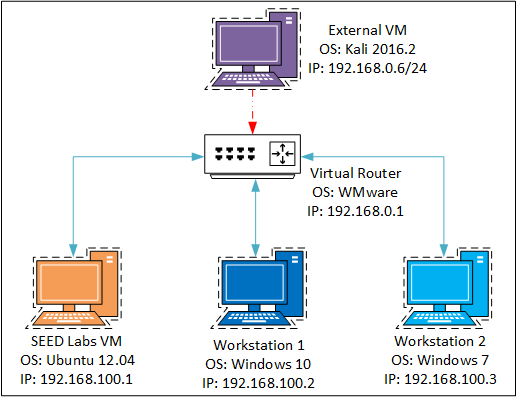
\includegraphics{NetworkDiagram.png}
		\end{center}
		
		
		\pagebreak
		\vspace{8mm}
		\item \textbf{Change-Log:}
		\label{changelog}
		
		\vspace{6mm}
		
		\begin{tabular}{ |p{1cm}|p{3cm}|p{4cm}|p{7cm}|  }
			\hline
			\multicolumn{4}{|c|}{Network Protocol Analysis with Wireshark tutorial} \\
			\hline
			\texttt{\textbf{Ver.}} & \texttt{\textbf{Date}} & \texttt{\textbf{Authors}} & \texttt{\textbf{Changes}} \\
			\hline
			v1 & Feb. 1st 2016 & Jon Meyer and Jared Zook & First draft of tutorial. \\
			\hline
			v2 & July 6th 2016 & Ananth Jillepalli & Major content additions and remodeled the structure. \\
			\hline
			v2.1 & July 13th 2016 & Ananth Jillepalli & Added the `Appendix' section and other minor enhancements. \\
			\hline
			v3 & Jan. 29th 2017 & Robert Breckenridge & Added Observations: Capture Options, Activity: Capture Filters, Question: Capture Filters, Activity: Live Capture, and Challenge IV-VII. Updated Hardware and Software Requirements and adjusted some formatting throughout the document. \\
			\hline
			v3.1 & Jan. 30th 2017 & Matthew Holman & Updated/ edited wording throughout the entire document for increased clarity. \\
			\hline
			v3.2 & July 1st 2017 & Ananth Jillpalli & Standardization (network layout diagram edits, consistency, TeX markup cleaning, and more)  \\ \hline
			\end{tabular}
	
	\end{enumerate}
		
		
	%------------------------------------------------------------------------------------------------------------------------------------------------------------------------------------------------------------------%
	
	\pagebreak
	\addcontentsline{toc}{section}{References}
	%\bibliographystyle{plain}
	\bibliographystyle{IEEEtran}
	\bibliography{bibfile}
	
	% this style of bibliography shows urls
	%\bibliographystyle{IEEEtran}
	%\begin{thebibliography}{9}
		%example biblio entry
		%\iffalse
		%\bibitem{Winkler15}
		%    Winkler, I.
		%    2015
		%    \textit{The 'Sophisticated Attack' Myth}\\, page accessed January 2016.
		%    ComputerWorld, The Internet, 2015.
		%\fi 
	%\end{thebibliography}
	

\end{document}